In the previous section, we showed that there are two margins on which clustering methodologies are sensitive:  uncertainty in the input data and the choice of the number of clusters. However, these issues are only important for empirical labor economists to the extent that these sensitivities impact empirical estimates in a meaningful way. To that end, in this section, we demonstrate the impact these issues have on empirical estimates. 

In our analysis, we consider the effect that changes in local labor demand have on receipts of unemployment insurance in the local area. To estimate this effect, we measure labor demand using a standard Bartik measure, which can be expressed by the equation below, and is very similar to \citet{Bartik1991}.\footnote{Other papers that use this measure of labor demand include \citet{BH2000} and \citet{Notowidigdo2011}.}


\begin{equation}\label{eqn:bartik}
Demand_{k,t} = \sum_{s} \frac{Emp_{ks,1990}}{Emp_{k,1990}} (log(Emp_{s,t}) - log(Emp_{s,t-1}))
\end{equation}

The above equation states that demand for area, or cluster, $k$ in year $t$ is a weighted sum over the industry sectors $s$, where the weights are the original period employment distribution in an area. Given the employment distribution, the national changes in employment in industry $s$ ($log(Emp_{s,t}) - log(Emp_{s,t-1})$) affect some areas more, based on how much employment was originally in that industry and area.

To measure all the components of Equation \ref{eqn:bartik}, we use the Quarterly Census of Employment and Wages from the Bureau of Labor Statistics from 1991-2015, and for all the employment measures we use average annual employment for each of the twenty NAICS industry sectors. Additionally, we measure the total receipts of unemployment insurance using the BEA's Regional Economic Accounts data.
%https://www.bea.gov/regional/definitions/
%Is this data on Github? I could not find. It should have all the series names.

Our estimating equation is as follows:\footnote{This analysis is similar to \citet{ADH2013} and \citet{Notowidigdo2011}, who both look at how labor demand changes affect receipt of public assistance.}

\begin{equation}\label{eqn:bartikreg}
log(UIReceipts)_{i,t} = \beta Demand_{i,t-1} + \gamma_i + \delta_t+ \epsilon_{i,t}
\end{equation}

Where $Demand_{it}$ is measured according the equation \ref{eqn:bartik}, and $\gamma_i$ and $\delta_t$ are area and year fixed effects. Initially, we estimate this equation only for the original commuting zone definitions from Tolbert and Sizer and our replication. In the subsequent subsection, we then present estimates using different realizations of commuting zones based on the results from Section \ref{sec:dsens}.

\subsection{Results of Estimating Equation}
\FloatBarrier

\begin{table}[tbh]\centering
\caption{Effect of Labor Demand on Unemployment Receipt \label{tab:bartik_results}}
\begin{tabular}{lcc}
\hline\hline
       & Using TS1990 CZs & Using FKV1990 CZs \\
       	
       \hline
$Demand_{it}$ & -5.409 & -6.643  \\
              & (0.686) & (0.5904) \\
\hline
N			&	18441	&	20058	\\
R-squared 	&	0.983	&	0.976	\\

\hline
\multicolumn{3}{p{4in}}{\footnotesize \textit{Notes}: Table from author's calculations, based on equation \ref{eqn:bartikreg}. Column 1 uses Tolbert and Sizer's commuting zone definitions, while Column 2 uses replicated commuting zones from Section \ref{sec:dsens}. Standard errors in parentheses are clustered at the commuting zone level. All coefficients are significant with p-values less than 0.01.}\\
\end{tabular}
\end{table}

Our results in Table \ref{tab:bartik_results} show that when labor demand increases, unemployment receipts fall.\footnote{Observations approximately equal the product of 25 years by the number of clusters in each definition. A few observations are missing due to missingness in certain states for the early period in the BEA data.} To scale our results, a one standard deviation change in labor demand (0.02) causes unemployment receipts to fall by approximately 10 percent.

The results are slightly different depending on which set of commuting zone definitions are used, with our replicated CZs yielding a more negative result. Both are significant, but this fact highlights that results can be sensitive to the definition of local labor markets used in analysis.

\subsection{Sensitivity to Chosen Cutoff}

In Section \ref{sec:dsens} we showed that the decision of where to stop the clustering process was rather arbitrary, since there is no clear guidance on what cutoff is most appropriate. To demonstrate how the cutoff choice affects estimates of $\beta_1$ from Equation \ref{eqn:bartikreg}, we generate clusters based on cutoffs between 0.9 and 0.97 and estimate the equation using the resulting clusters. The count of clusters in this range falls from 1,423 to 303, so observations drop and the standard errors rise with the cluster height cutoff. Again, we not that starting closely after our chosen cutoff for replication, a large cluster forms that is not consistent with our interpretation of local labor markets. For this reason, we take the estimates for lower cutoff values to be more reasonable.

\begin{figure}\centering
\caption{Differences in Effect Based on Cluster Cutoff \label{fig:cutoff_dist}}
\begin{tabular}{c}

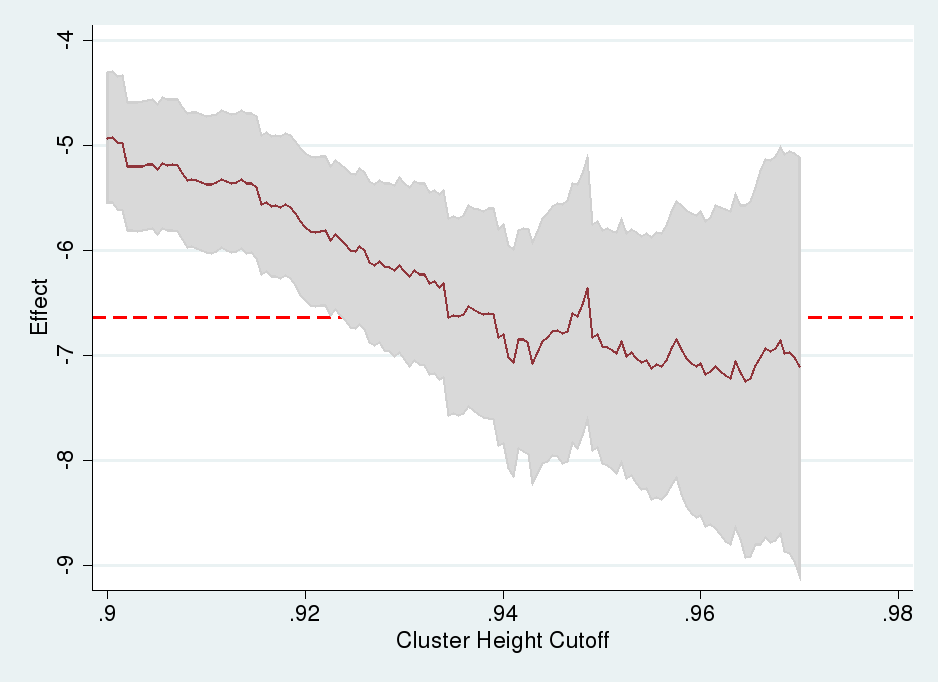
\includegraphics[scale=.35]{./figures/cutoff_bartik.png} \\ 

\multicolumn{1}{p{6.5in}}{\footnotesize \emph{Note:} Author's estimates of $\beta$ in Equation \ref{eqn:bartikreg} based on replication of Tolbert and Sizer's method while varying the cluster height cutoff. The solid red line gives the point estimate for the cluster definitions at each height and the gray area denotes the 90 percent confidence interval including the estimate. The red dashed line gives the point estimate for clusters using the definition FKV1990.}
\end{tabular}
\end{figure}

Figure \ref{fig:cutoff_dist} displays the results of this exercise. Again, our results show that there is some variation in the estimate based on the cutoff value. As the cutoff increases (and there are fewer areas) the effect becomes more negative. However, the relationship is not monotonic.

\subsection{Sensitivity to Errors in Flows Data}

To demonstrate how sensitive the results of Equation \ref{eqn:bartikreg} are to different commuting definitions, we re-estimate the equation using the 1000 realizations of commuting zones that were generated in the previous section.

\begin{figure}\centering
\caption{Distribution of Effect \label{fig:1990dist}}
\begin{tabular}{c}
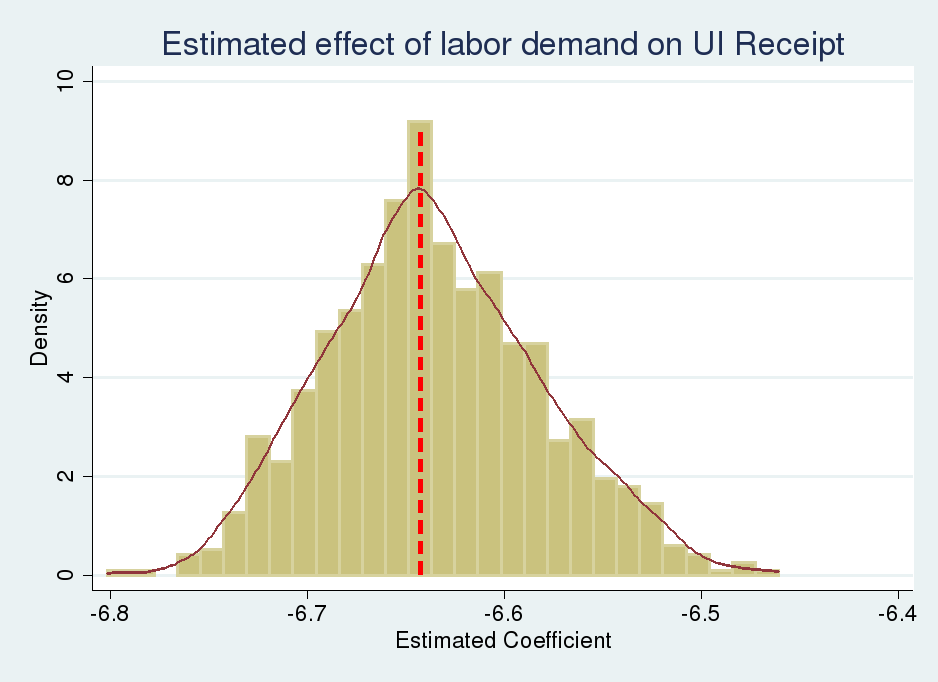
\includegraphics[scale=.35]{./figures/beta_bartik_distribution_moe_new.png}\\
\multicolumn{1}{p{4.5in}}{\footnotesize \emph{Note:} Histogram plots estimates of $\beta_1$ from equation \ref{eqn:bartikreg}, based on commuting zone realizations as outlined in Section \ref{sec:dsens}. Red vertical line shows estimates using replicated commuting zones.}
\end{tabular}
\end{figure}

 The coefficients from this exercise are graphed in Figure \ref{fig:1990dist}, which shows the distribution of the estimated effect from our exercise. The red vertical line shows the estimate using the published flows data from our national replication. Approximately 95 percent of the estimates are within 0.1 of the point estimate -6.643 for FKV1990.

Another way to summarize the results of this exercise is to look at the distribution of t-statistics, which incorporates information about the standard error of $\beta$ into the analysis as well, and comparing that distribution to the critical values. To use the distribution of t-statistics in an empirical setting, researchers construct a 95\% confidence interval of the t-statistic by using the values at the 97.5th and 2.5th percentiles of the 1000 realizations. If this confidence interval is outside the critical value $t_{0.025}$, then the null hypothesis can be rejected at $\alpha = 0.05$. 

To give an empirical application, Figure \ref{fig:1990_tdist} shows the distribution of t-statistics obtained from estimating Equation \ref{eqn:bartikreg}. The blue vertical line is the original t-statistic, and the light gray vertical lines are the 2.5th and 97.5th percentiles. Clearly, in this application the result is still significant, because the entire confidence interval of t-statistics is less than the critical value ($-1.96$). Once again, the t-statistic from the original estimate is one of the smallest in magnitude.

Importantly, the estimated t-statistic from the original regression (blue vertical line) is not the center of the distribution. While this is not true in all applications, it warrants caution on the part of the researcher, because the zones that are used by the researcher may represent an outlier in terms of statistical significance.

\begin{figure}\centering
\caption{Distribution of T-Statistic \label{fig:1990_tdist}}
\begin{tabular}{c}
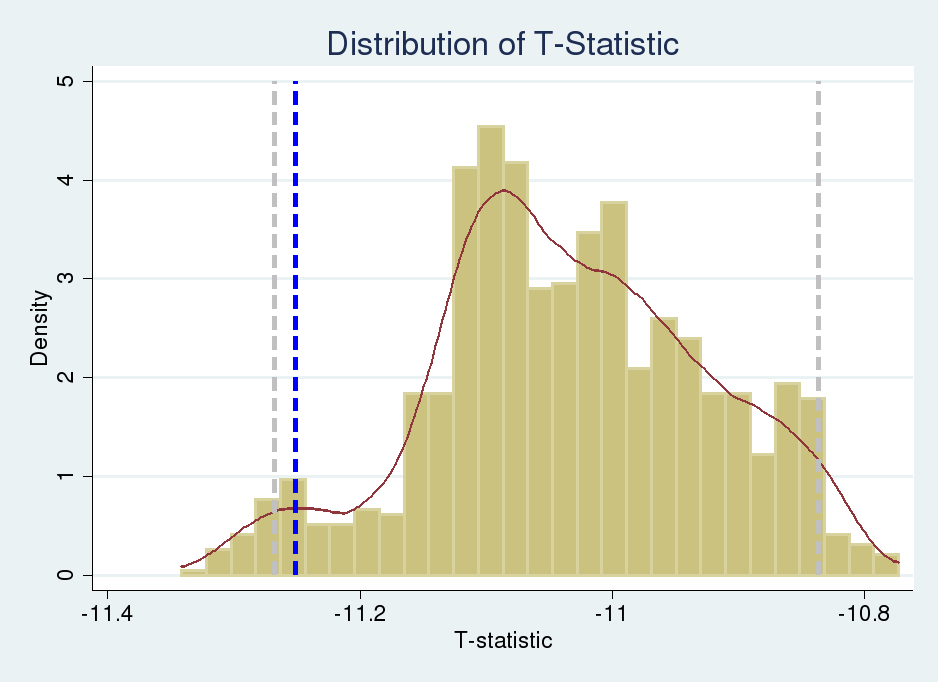
\includegraphics[scale=.35]{./figures/tdistribution_bartik_moe_new.png}\\
\multicolumn{1}{p{4.5in}}{\footnotesize \emph{Note:} Histogram plots t-statistics derived from estimating  equation \ref{eqn:bartikreg}, based on commuting zone realizations as outlined in Section \ref{sec:dsens}. Blue vertical line is t-statistic using FKV1990, and gray vertical lines are the 2.5th and 97.5th percentiles of the t-statistic distribution.}
\end{tabular}
\end{figure}

This exercise demonstrates that there is additional uncertainty induced by the construction of the commuting zones that is not addressed in empirical estimates that use these definitions, which may overstate the precision of the results.





